\documentclass[parskip=half]{scrartcl}

% packages %%%%%%%%%%%%%%%%%%%%%%%%%%%%%%%%%%%%%%%%%%%%%%%%%%%%%%%%%%%
\usepackage[T1]{fontenc}	
\usepackage[utf8]{inputenc}		
\usepackage[english]{babel}
\usepackage[bitstream-charter]{mathdesign}
\usepackage{tikzducks}
\usepackage[most]{tcolorbox}
\usepackage[paper=a4paper,margin=3cm]{geometry}
\usepackage[colorlinks=true,breaklinks=true,urlcolor=duckblue,linkcolor=duckblue,citecolor=duckblue,filecolor=duckblue]{hyperref}

% customisation %%%%%%%%%%%%%%%%%%%%%%%%%%%%%%%%%%%%%%%%%%%%%%%%%%%%%%
\definecolor{duckblue}{RGB}{0,70,140}
\addtokomafont{sectioning}{\color{duckblue}}
\addtokomafont{date}{\normalsize}
\addtokomafont{author}{\normalsize}

\tcbset{%
	colframe=duckblue,
	arc=2mm,
	fonttitle=\bfseries,
	sidebyside,
	listing options={%
		language={[latex]TeX},
		tabsize=2,
		breaklines,
		basicstyle=\footnotesize\ttfamily,
		commentstyle={\color{green!50!black}\slshape}, 
		columns=fullflexible,
		texcsstyle=*\color{duckblue}\bfseries,
		keywordstyle=\color{red!60!black}\bfseries,
		morekeywords={tikzpicture,scope},
		moretexcs={duck,path,definecolor,duckpathjacket,duckpathbody,duckpathgrumpybill,duckpathbill,duckpathtshirt,duckpathshorthair,duckpathlonghair,duckpathcrazyhair,duckpathrecedinghair,scalebox,foreach,node},
	  delim ={[s][\ttfamily\color{green!50!black}]{$}{$}}
	},
	righthand width=6.5cm
}

% meta %%%%%%%%%%%%%%%%%%%%%%%%%%%%%%%%%%%%%%%%%%%%%%%%%%%%%%%%%%%%%%%
\title{The \texorpdfstring{\texttt{tikzducks}}{tikzducks} package}
\subtitle{using ducks in tikz}
\author{%
	\texorpdfstring{\texttt{samcarter} (alias 
		
\begin{tikzpicture}[scale=0.3,baseline=5pt]
			\duck[body=yellow!50!brown!50!white,
					longhair=red!50!brown, 
					jacket=blue!50!black]
		\end{tikzpicture})\\[0.8em]
		\url{https://github.com/samcarter8/tikzducks}\\
		\url{https://www.ctan.org/pkg/tikzducks}
	}{samcarter}}
\date{Version 0.2 -- \today}

\begin{document}

\maketitle
\section{Introduc(k)tion}
\label{intro}

The \verb|tikzducks| package is a latex package for ducks to be used in \verb|tikz| pictures. 
This project is a continuation of an answer at TeX.Stackexchange: \href{tex.stackexchange.com/a/347458/36296}{How can we draw a duck?}.

This package is work in progress (and will probably never be really finished as there is an infinite amount of things which could be added), therefore I would be happy to hear your feedback and ideas how to improve the package. 
The head version of the source code can be found on \url{github.com/samcarter8/tikzducks}, including a bug tracker, please make constructive use of it! A more stable package version can be found on ctan (\url{www.ctan.org/pkg/tikzducks}) and is included in both
miktex and texlive as \verb|tikzducks|. 

\subsection{Acknowledgements}

Without the friendly and helpful community of \href{https://tex.stackexchange.com/}{TeX.Stackexchange} this package would not exist. I would like to thank a few fellow users in particular:

First of all \href{https://tex.stackexchange.com/users/101651/carlatex}{CarLaTeX} for pointing out the overwhelming need of having a \verb|tikzducks| package and \href{https://tex.stackexchange.com/users/3094/paulo-cereda}{Paulo Cereda} for his contagious enthusiasm for ducks (\emph{Quack!}). Many other users contributed to this package (in random order): \href{https://tex.stackexchange.com/users/4427/egreg}{egreg} helped to implement the \verb|\tikzset{}| interface which makes it much easier to adjust the properties of the ducks to fit the user needs, \href{https://tex.stackexchange.com/users/51022/symbol-1}{Symbol 1}  solved a few problems with default key values, \href{https://tex.stackexchange.com/users/2388/ulrike-fischer}{Ulrike Fischer} gave valuable \verb|tikz| advices and last but not least my thanks go to \href{https://tex.stackexchange.com/users/5763/martin-schr%c3%b6der}{Martin Schr\"oder} for his feedback to the code review.

The ducks mostly consist of basic geometric shapes drawn in \verb|tikz|. Some of the more complex shapes (e.g.\ the different hair styles) are first drawn in \verb|inkscape|\footnote{\url{inkscape.org}} and then exported to \verb|tikz| paths using the \verb|SVG to TikZ/PGF| extension\footnote{\url{github.com/kjellmf/svg2tikz}}

\subsection{Dependencies}

The \verb|tikzducks| package loads the packages \verb|xcolor| and \verb|tikz|, both without any options. If you require one of these packages to be loaded with some option, please consider loading it yourself before the \verb|tikzducks| package or use, e.g.

\verb|    \PassOptionsToPackage{svgnames}{xcolor}|

It also uses the \verb|\usetikzlibrary{patterns}|.

\subsection{License}

Copyright \raisebox{0.2em}{\tiny\fontfamily{cmr}\selectfont\textcopyright}
\verb|samcarter|. Permission is granted to copy, distribute and\slash or modify this software under the terms of the LaTeX project public licence, version 1.3c or later \url{http://www.latex-project.org/lppl.txt}.

The shown example ducks are purely fictional characters, any resemblance to real ducks or persons is purely coincidental and no copyright infringement is intended.

\section{Usage}

The basic usage is fairly simple, to draw a duck:
\begin{tcblisting}{title={Basic duck}}

\begin{tikzpicture}
	\duck
\end{tikzpicture}
\end{tcblisting}

To customise this basic duck, the package uses \verb|pgf| keys. For almost all parts the colour can be changed using \verb|<shape name>=<colour name>|. For example to change the colour of the duck:
\begin{tcblisting}{title={Blue duck}}
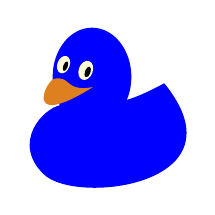
\begin{tikzpicture}
	\duck[body=blue]
\end{tikzpicture}
\end{tcblisting}

\clearpage
If the size of the ducks should be changed or shifted:
\begin{tcblisting}{title={Scaled duck},	righthand width=3cm}
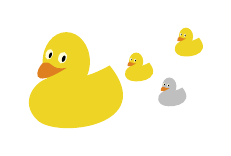
\begin{tikzpicture}[scale=0.6]
	\duck
	\begin{scope}[xshift=90pt, scale=.3, yshift=150pt]
		\duck
	\end{scope}
	\begin{scope}[xshift=60pt, scale=.3, yshift=100pt]
		\duck
	\end{scope}
	\begin{scope}[xshift=80pt, scale=.3, yshift=50pt]
		\duck[body=gray!50!white,head=gray!50!white]
	\end{scope}		
\end{tikzpicture}
\end{tcblisting}

\subsection{Body parts}

The various parts of the duck body can also be coloured independently, i.e. \verb|body|, \verb|head| or \verb|bill|:
\begin{tcblisting}{title={Harlequin duck}}
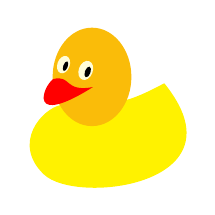
\begin{tikzpicture}
	\duck[body=yellow,
		head=yellow!50!orange, 
		bill=red]
\end{tikzpicture}
\end{tcblisting}

Furthermore using the keyword \verb|grumpy| the shape of the bill can be changed:
\begin{tcblisting}{title={Grumpy duck}}

\begin{tikzpicture}
	\duck[grumpy]
\end{tikzpicture}

\begin{tikzpicture}
	\duck[grumpy, bill=cyan]
\end{tikzpicture}
\end{tcblisting}

\clearpage
\subsection{Hair styles}

Some duck also like to have nice hair cuts, several different hair styles are available:
\begin{tcblisting}{title={Hairy duck}}

\begin{tikzpicture}
	\duck[longhair]
\end{tikzpicture}

\begin{tikzpicture}
	\duck[shorthair]
\end{tikzpicture}

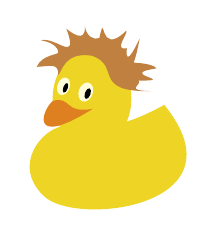
\begin{tikzpicture}
	\duck[crazyhair]
\end{tikzpicture}

\begin{tikzpicture}
	\duck[recedinghair]
\end{tikzpicture}
\end{tcblisting}

And of course the colour of each hair style can be adjusted:
\begin{tcblisting}{title={Coloured hair duck}}

\begin{tikzpicture}
	\duck[longhair=teal]
\end{tikzpicture}
\end{tcblisting}

Eyebrows are also part of the package. The colour choice is more tricky for them -- if a colour is explicitly specified \verb|eyebrow=<colour name>| this colour is of course used, but if no colour is given, it first falls back to the hair colour and only if the duck does not have any hairs, the default colour is applied.
\begin{tcblisting}{title={Eye brow duck}}

\begin{tikzpicture}
	\duck[eyebrow]
\end{tikzpicture}
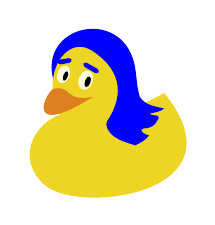
\begin{tikzpicture}
	\duck[longhair=blue, 
		eyebrow]
\end{tikzpicture}

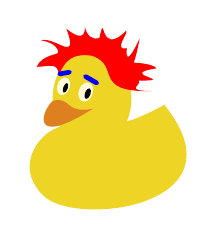
\begin{tikzpicture}
	\duck[crazyhair=red, 
		eyebrow=blue]
\end{tikzpicture}
\end{tcblisting}

\subsection{Clothing}

A respectable duck needs a suitable wardrobe. It can choose from a \verb|tshirt|, a \verb|jacket| and a \verb|tie|. In it's infinite wardrobe these items are available in all colours definable in the current colour model.
\begin{tcblisting}{title={Dressed duck}}
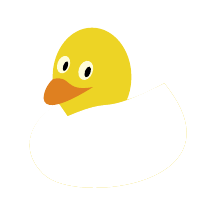
\begin{tikzpicture}
	\duck[tshirt]
\end{tikzpicture}
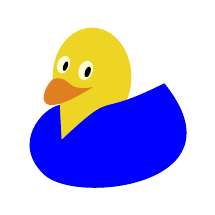
\begin{tikzpicture}
	\duck[jacket]
\end{tikzpicture}

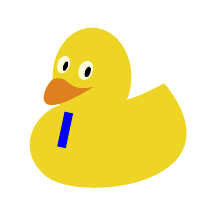
\begin{tikzpicture}
	\duck[tie]
\end{tikzpicture}
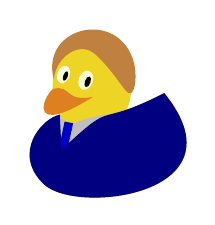
\begin{tikzpicture}
	\duck[tshirt=lightgray, 
			jacket=blue!50!black, 
			tie=blue!80!black, 
			shorthair]
\end{tikzpicture}
\end{tcblisting}

\subsection{Accessoires}

There is a multitude of things a duck might need. 

The following examples all also work without specifying a colour, but giving an examples with and one without explicit colour just makes this overview unnecessary long, so only one is given.

\begin{tcblisting}{title={Swimming duck}}
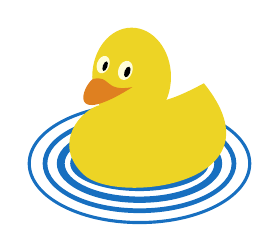
\begin{tikzpicture}
	\duck[water=cyan!50!blue]
\end{tikzpicture}
\end{tcblisting}

\begin{tcblisting}{title={Alien duck}}
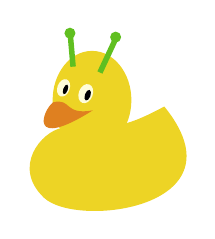
\begin{tikzpicture}
	\duck[alien=green!50!brown]
\end{tikzpicture}
\end{tcblisting}

\begin{tcblisting}{title={Hat duck}}
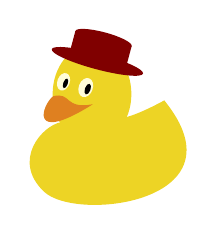
\begin{tikzpicture}
	\duck[hat=red!50!black]
\end{tikzpicture}
\end{tcblisting}

\begin{tcblisting}{title={Basecap duck}}
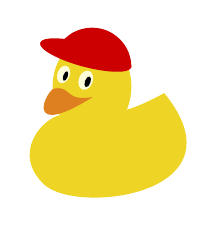
\begin{tikzpicture}
	\duck[cap=red!80!black]
\end{tikzpicture}
\end{tcblisting}

\begin{tcblisting}{title={Santa Clause}}

\begin{tikzpicture}
	\duck[santa=red!80!black]
\end{tikzpicture}
\end{tcblisting}

\begin{tcblisting}{title={Unicorn duck}}
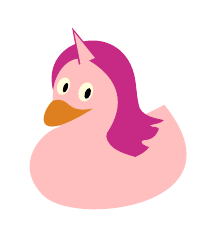
\begin{tikzpicture}
	\duck[body=pink,
		unicorn=magenta!60!violet,
		longhair=magenta!60!violet]
\end{tikzpicture}
\end{tcblisting}

\begin{tcblisting}{title={Glasses duck}}
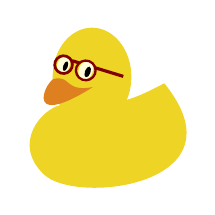
\begin{tikzpicture}
	\duck[glasses=red!50!black]
\end{tikzpicture}
\end{tcblisting}

\begin{tcblisting}{title={Sunglasses duck}}

\begin{tikzpicture}
	\duck[sunglasses=blue]
\end{tikzpicture}
\end{tcblisting}

\begin{tcblisting}{title={Book duck}}

\begin{tikzpicture}
	\duck[book=\scalebox{0.5}{\TeX}]
\end{tikzpicture}

\begin{tikzpicture}
\duck[book=\scalebox{0.6}{$\pi$}, bookcolour=blue!50!black]
\end{tikzpicture}
\end{tcblisting}

\begin{tcblisting}{title={Magic duck}}

\begin{tikzpicture}
	\duck[magichat,
				magicwand]
\end{tikzpicture}

\begin{tikzpicture}
	\duck[magichat=teal,
				magicstars=blue!30!cyan,
				magicwand]
\end{tikzpicture}
\end{tcblisting}

\begin{tcblisting}{title={Cricket duck}}

\begin{tikzpicture}
	\duck[cricket=red!50!black]
\end{tikzpicture}
\end{tcblisting}

\begin{tcblisting}{title={Icecream duck}}

\begin{tikzpicture}
	\duck[icecream]
\end{tikzpicture}

\begin{tikzpicture}
	\duck[icecream=brown, flavoura=brown, flavourb=white, flavourc=red]
\end{tikzpicture}
\end{tcblisting}

\clearpage
\section{Further customisation}

This package will never be able to do everything every potential user might want to do, as this number quickly approaches $\infty$ -- but as the ducks are simply things inside \verb|tikzpicture|s, all the heavy weapons of the \verb|tikz| package are available for further customisation.

\begin{tcblisting}{title={Adding things to the duck}}
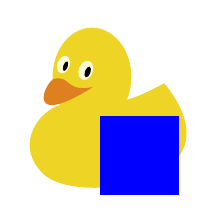
\begin{tikzpicture}
\duck
\fill[blue] (2,0) rectangle (1,1);
\end{tikzpicture}
\end{tcblisting}

\begin{tcblisting}{title={Monochrome duck}}
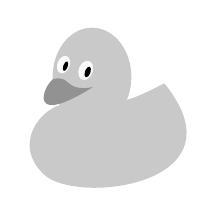
\begin{tikzpicture}
\selectcolormodel{gray}
\duck
\end{tikzpicture}
\end{tcblisting}

For convenience the more complex paths of this package are stored in macros, which can easily be reused:
\begin{tcblisting}{title={Redraw parts}}
\begin{tikzpicture}
\duck
\path[preaction={fill, red!50!black},pattern=fivepointed stars, pattern color=yellow]  
\duckpathlonghair;
\end{tikzpicture}
\end{tcblisting}

In detail, the following paths are available: \verb|\duckpathbody|, \verb|\duckpathgrumpybill|, \linebreak\verb|\duckpathbill|, \verb|\duckpathtshirt|, \verb|\duckpathjacket|, \verb|\duckpathshorthair|, \hbadness10000\linebreak\verb|\duckpathlonghair|, \verb|\duckpathcrazyhair|, \verb|\duckpathrecedinghair|. In case one of the other shapes is needed, please have a look at the source code in \verb|tikzducks.sty|.

\clearpage
\section{Examples}

\begin{tcblisting}{title={\texttt{samcarter} duck},	righthand width=3cm}
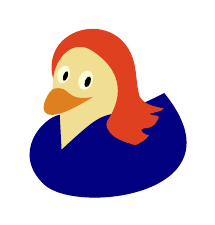
\begin{tikzpicture}
	\duck[body=yellow!50!brown!50!white, 
		longhair=red!50!brown, 
		jacket=blue!50!black]
\end{tikzpicture}
\end{tcblisting}

\begin{tcblisting}{title={Paulo duck}, righthand width=3cm}
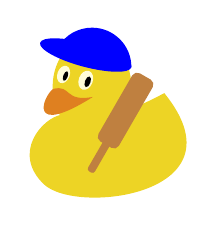
\begin{tikzpicture}
	\duck[cap,cricket]
\end{tikzpicture}
\end{tcblisting}

\begin{tcblisting}{title={Brazil duck},	righthand width=3cm}
\begin{tikzpicture}
\definecolor{brazilgreen}{RGB}{0,155,58}
\definecolor{brazilyellow}{RGB}{254,223,0}
\definecolor{brazilblue}{RGB}{0,39,118}
	\duck[body=brazilyellow,
				shorthair=brazilgreen]
	\path[preaction={fill, brazilblue},pattern=fivepointed stars, pattern color=white] 
	\duckpathjacket;
\end{tikzpicture}
\end{tcblisting}

\begin{tcblisting}{title={Duck in black},	righthand width=3cm}

\begin{tikzpicture}
	\duck[grumpy, body=yellow!50!brown!50!white, tshirt=white, jacket=black, tie=black, hat=black, sunglasses=black]
\end{tikzpicture}
\end{tcblisting}

\begin{tcblisting}{title={Prof.\ van Duck}, righthand width=3cm}

\begin{tikzpicture}
	\duck[body=yellow!50!brown!40!white,
		crazyhair=gray!50!white,
		eyebrow,
		glasses=brown!70!black,
		book=\scalebox{0.2}{$E=mc^2$},
		bookcolour=red!20!brown]
\end{tikzpicture}
\end{tcblisting}

\begin{tcblisting}{title={Knuth duck},	righthand width=3cm}
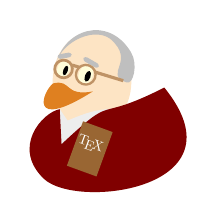
\begin{tikzpicture}
	\duck[body=yellow!50!red!20!white,
		recedinghair=gray!50!white,
		eyebrow,
		tshirt=white!93!black,
		jacket=red!50!black,
		glasses=brown!70!lightgray,
		book=\scalebox{0.5}{\TeX},
		bookcolour=black!20!brown]
\end{tikzpicture}
\end{tcblisting}

\addtocounter{footnote}{1}
\begin{tcblisting}{title={67P/Churyumov-Gerasimenko duck$^\thefootnote$},	righthand width=3cm}
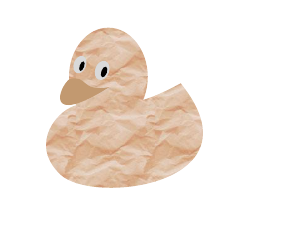
\begin{tikzpicture}[path image/.style={path picture={\foreach \j in {0,...,2}{\node at (0,\j) {\foreach \i in {1,...,5}{\includegraphics[height=1cm]{#1}}};}}}]
\path [path image=crinklepaper] 
	(0.90,1.50) ellipse (0.50 and 0.625);
\path [path image=crinklepaper] \duckpathbody;
\fill [orange!40!gray!80!white]  \duckpathbill;
\fill[white!70!gray, rotate=-20]
	(0.23,1.7675) ellipse (0.0893 and 0.125);
\fill[black, rotate=-20]
	(0.26,1.7575) ellipse (0.0357 and 0.0714);
\fill[white!70!gray, rotate=-20]
	(-0.06,1.74) ellipse (0.0786 and 0.1143);
\fill[black, rotate=-20]
	(-0.03,1.73) ellipse (0.0286 and 0.0643);
\end{tikzpicture}
\end{tcblisting}
\footnotetext[\thefootnote]{If you try this at home, replace the \texttt{crinklepaper} with an image of the comet's surface, e.g. \url{arxiv.org/abs/1707.02945}}

\end{document}